\section{Lab 1}
\label{sec:lab1}
In this laboratory assignment, we evaluate overheads in cache coherence protocols using microbenchmarks. Three diverse benchmarks, described in section \ref{sec:lab11}, are used to compare the coherence protocols. In section \ref{sec:lab12}, MSI and MESI is compared and in section \ref{sec:lab13}, MESI and MESI-MG is compared. In each comparison, we use three working set: the first is smaller than an private L1 cache (512 counters), the second is larger than an private L1 cache and smaller than the LLC (1536 counters), and the last is larger than the LLC (98304 counters). The counters are stored in an array, the counter array, which is accessed by the benchmark.

\subsection{Task 1}
\label{sec:lab11}
Three different microbenchmarks with disgustingly various communication patterns are used in the simulations and here follow a description of each.
\subsubsection*{Benchmark 1 - Producer consumer}
In this benchmark, one thread increments the values in the counter array, whereas the other threads read these values and accumulate the read values in a private variable. However, it is not ensured that the incrementing thread increments the values before the other threads reads, and thus can this happen in any order. A counter access is done in mutual exclusion using a lock, and before a new lap of increments \& reads there is a barrier.

\subsubsection*{Benchmark 2 - No sharing}
This benchmark have no sharing of the counter array. The counter array is divided up equally among the threads, giving each thread access to every nth counter element, where n is the number of threads. Each thread then increments it's assigned counters sequentially. A barrier is placed before a new incrementation lap of the assigned array elements begin. 

\subsubsection*{Benchmark 3 - All shared}
In this benchmark, the counter array is shared among all threads. Each thread increments every element in the counter array sequentially while in mutual exclusion. A lock is used to provide mutual exclusion and a barrier is placed before a new incrementation lap. 

\subsection{Task 2}
\label{sec:lab12}
Here the CCPs MSI and MESI are compared using benchmark 1 and 2. The difference between the CCPs is that MESI includes an exclusive (E) state, which is beneficial if data is read exclusively by one processor. If the data is then read by another processor, a move to the shared (S) state is made without cost. I.e. MESI can only produce equal or better results than MSI.

In the producer consumer benchmark, the E state is beneficial if the writing thread accesses the data element for the first time or when it has been fetched from higher level caches. Then, the thread will transition the data element from I to M through E, when performing an increment. This avoids the S state, which give an increased performance as no bus command has to be issued. However, the probability that the writing thread accesses the data first is low, $\frac{1}{nthreads}$, which is shown in \reffig{fig:lab1bars} where MSI and MESI seems to perform equally. As the working set size increases, the benefit of the E state increases due to more frequent reads from globally invalid cache lines. This can however not be seen in the simulation results, due to fluctuations.

In the no sharing benchmark the first read access to every element end in state S for MSI and state E for MESI, respectively. The following write transitions the element to state M for both the CCPs, but MSI have to issue a BusUpdate whereas MESI's transition is costless. The BusUpdate broadcasts an invalidate signal which gives MSI a slight reduction in performance compared to MESI. In the small working set the elements will stay in state M to the end of execution, but in working sets larger than a private L1 cache the element has to be fetched from higher levels. This makes MSI issue an invalidate broadcast for each increment and the accumulated overhead is easily spotted in \reffig{fig:lab1bars}. 

\begin{figure}[t]
	\center
	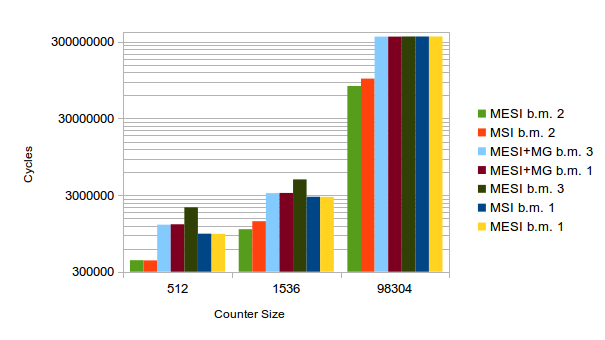
\includegraphics[width=0.7\textwidth]{lab1bars}
	\caption{Simulation results using various cache coherence protocols combined with different working sets and benchmarks.}
	\label{fig:lab1bars}
\end{figure}

\subsection{Task 3}
\label{sec:lab13}
MESI is here compared with MESI-MG by executing benchmark 1 and 3. MESI-MG is a modified version of MESI where the S state is not utilized; if a cache issues a read request of a data element which exists in state E or M in a remote cache, the data is forwarded from the remote cache and then the remote cache invalidates it's copy. By this scheme, the S state is never used.

The producer consumer benchmark benefit from the S state, and therefor produces MESI better results than MESI-MG. In the benchmark, one thread update an element whereas the other threads read it and by migrating the element from one private cache to the other is less optimal than letting the reading threads share the element and read it in parallel. This overhead will be a smaller part of the total cycles as the working set increases, as the misses increase in the private caches and also in the LLC, which is costly in terms of cycles. This trend is shown in \reffig{fig:lab1bars}. 

In the all shared benchmark, every thread increments every data element in mutual exclusion which favors MESI-MG. Each data element is read and modified exclusively by one processor at a time, thus is the S state not beneficial. As MESI-MG do not utilize the S state, as described, it is more suitable than MESI in this benchmark. In Table \ref{tbl:lab1:task3} it is shown that the CCPs results are alike, except that MESI have to issue a significant number of invalidates, which is needed for the transition from state S to M. As shown in \reffig{fig:lab1bars}, MESI-MG's benefit is not visible for the working set size increasing the size of the LLC. That is because the cycle count is dominated by the LLC misses, as in the producer consumer benchmark.